\begin{center}
Problema H

Josephus das Abóboras

{\small Nome do arquivo: H.c, H.cpp, H.java, ou H.py}

{\large Timelimit: $1$}

{\tiny Por Heverton Barros de Macêdo}

\end{center}

{\footnotesize
Finalmente chegou o dia das bruxas e os “corajosos” estudantes de Ciência da Computação estão prontos para adentrar no castelo mal-assombrado. O problema é que a porta do castelo é muito estreita e permite que apenas um estudante adentre por vez. Como todos estão com medo, Josephus decidiu fazer um sorteio para estabelecer a ordem em que eles devem entrar. A seguinte regra foi estabelecida:

\begin{enumerate}
    \item Os estudantes devem se posicionar em formato de círculo;
    \item Cada estudante apresenta um número com os dedos da mão;
    \item Faz-se a soma dos números e define o resultado como X;
    \item A contagem dos estudantes é iniciada em zero a partir do primeiro estudante adicionado no círculo, seguindo em sentido horário. Quando a contagem atingir X, o estudante daquela posição será escolhido como o primeiro a ingressar no castelo.
    \item O estudante seguinte ao escolhido, servirá como ponto de partida para a nova contagem até o número X, que determina o próximo a ingressar no castelo.
    \item O passo anterior deverá ser repetido até que reste apenas um estudante, momento em que a sequência é finalizada, definindo o último aluno a ingressar no castelo.
\end{enumerate}

Como exemplo, considere os estudantes: Fulano, Beltrano, Sicrano e Josephus. A disposição dos estudantes colocando-os em círculo pode ser visualizada na Figura \ref{figura:h1}.

\begin{figure}[!ht]
\centering
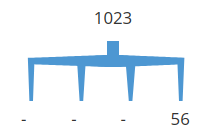
\includegraphics[width=8cm]{fig/h_1.png}
\caption{Disposição inicial em formato circular}
\label{figura:h1}
\end{figure}

Considere que a soma dos números dos dedos da mão indicados pelos estudantes seja 7 $(X = 7)$. Fazendo a contagem no sentido horário, partindo de Fulano, temos: Beltrano (1), Sicrano (2), Josephus (3), Fulano (4), continuando o círculo, Beltrano (5), Sicrano (6), Josephus (7). A Figura \ref{figura:h2} ilustra a contagem, destacando o número 7 em vermelho como sendo o estudante a ser removido do círculo.

\begin{figure}[!htbp]
\centering
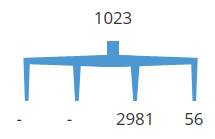
\includegraphics[width=8cm]{fig/h_2.png}
\caption{Contagem considerando o número $X = 7$ e o aluno Fulano como referência para o início da contagem}
\label{figura:h2}
\end{figure}

Para essa rodada o Josephus foi selecionado como primeiro a ingressar no castelo. Considerando Josephus fora do círculo, iniciamos novamente a contagem a partir do próximo do círculo (coincidentemente Fulano). Na sequência temos: Beltrano (1), Sicrano (2), Fulano (3), Beltrano (4), Sicrano (5), Fulano (6), Beltrano (7), indicando que Beltrano é o segundo a adentrar no Castelo. Continuando o sorteio com Beltrano fora do círculo e a contagem iniciando de Sicrano (próximo no sentido horário) teremos: Fulano (1), Sicrano (2), Fulano (3), Sicrano (4), Fulano (5), Sicrano (6), Fulano (7). Por fim, temos a sequência de estudantes a entrar no castelo: Josephus, Beltrano, Fulano e Sicrano.

Sua missão é ajudar Josephus a obter a sequência correta para adentrar ao castelo, independente do número de estudantes que estiver o acompanhando.

\vspace{0.3cm}
\textbf{Entrada:}
A entrada contém vários casos de teste. A primeira linha de cada caso contém os nomes dos estudantes separados com um espaço. A segunda linha contém o número inteiro X $(1 \leq X \leq 10.000)$ que será usado para a contagem (Obs: para cada nome não deve haver espaço e haverá no máximo 20 caracteres. Exemplo de nome inválido: "João da Silva". Exemplo de nome válido "JoãodaSilva").

\vspace{0.3cm}
\textbf{Saída:}
O programa deve produzir como saída a sequência de nomes a adentrar no castelo separados por um espaço (Obs: Ao término do último nome da lista não deve haver espaço, somente o terminador de linha).

\begin{table}[!htbp]
    \centering
    \begin{tabular}{|p{8cm}|p{7cm}|}
        \hline
        \begin{center}
            \vspace{-0.3cm}
            \textbf{Exemplos de Entrada}
            \vspace{-0.3cm}
        \end{center} 
         &  
        \begin{center}
            \vspace{-0.3cm}
            \textbf{Exemplos de Saída}
            \vspace{-0.3cm}
        \end{center} \\ \hline
         \texttt{Fulano Sicrano} & \texttt{Sicrano Fulano} \\  
         \texttt{1} & \texttt{} \\  
         \hline
         \texttt{Fulano Sicrano Beltrano} & \texttt{Sicrano Fulano Beltrano} \\  
         \texttt{1} & \texttt{} \\  
         \hline    
         \texttt{Fulano Sicrano Beltrano} & \texttt{Beltrano Fulano Sicrano} \\  
         \texttt{2} & \texttt{} \\  
         \hline
         \texttt{Fulano Sicrano Beltrano} & \texttt{Fulano Sicrano Beltrano} \\  
         \texttt{6} & \texttt{} \\  
         \hline
         \texttt{Fulano Beltrano Sicrano Josephus} & \texttt{Josephus Beltrano Fulano Sicrano} \\  
         \texttt{7} & \texttt{} \\  
         \hline 
    \end{tabular}
    \caption{Exemplos de entradas e saídas}
    \label{tab:inputHProblem24}
\end{table}}

\newpage

\begin{center}
\noindent
\lstinputlisting{abobora_24/H/H4.cpp}
\end{center}